\documentclass[10pt]{article}

\usepackage[utf8]{inputenc}
\usepackage[T1]{fontenc}
\usepackage{lmodern}
\usepackage[a4paper,margin=2.1cm]{geometry}
\usepackage{microtype}
\usepackage{amsmath,amssymb,mathtools}
\usepackage{graphicx}
\usepackage{booktabs,tabularx,array}
\usepackage{enumitem}
\usepackage{xcolor}
\usepackage{hyperref}
\usepackage[nameinlink,noabbrev]{cleveref}
\usepackage{natbib}
\usepackage{fancyhdr}
\usepackage{caption}
\usepackage{subcaption}
\usepackage{float}
\usepackage{listings}
\usepackage{url}

\definecolor{deepblue}{RGB}{30,70,110}
\definecolor{deepgreen}{RGB}{35,105,75}
\definecolor{deepred}{RGB}{145,45,45}
\definecolor{softgray}{RGB}{245,246,248}

\hypersetup{
  colorlinks=true,
  linkcolor=deepblue,
  citecolor=deepgreen,
  urlcolor=deepred,
  pdftitle={A Reproducible Tutorial on Synthetic-Data Scaling and Functional Collapse},
  pdfauthor={Guillaume Harbonnier},
  pdfsubject={Companion technical note for the synthetic-data scaling tutorial notebook}
}

\pagestyle{fancy}
\fancyhf{}
\lhead{Synthetic-Data Scaling Tutorial}
\rhead{Notebook Companion Note}
\cfoot{\thepage}
\setlength{\headheight}{14pt}
\setcounter{secnumdepth}{3}
\setcounter{tocdepth}{2}

\newcommand{\MMALS}{\textsc{MMALS}}
\newcommand{\STRATQ}{\textsc{STRAT-Q}}
\newcommand{\E}{\mathbb{E}}
\newcommand{\Prob}{\mathbb{P}}

\newenvironment{statusbox}{%
  \begin{center}\begin{minipage}{0.94\textwidth}\color{deepblue}\rule{\linewidth}{0.5pt}\par\vspace{0.3em}\noindent\textbf{Status.} }%
  {\par\vspace{0.3em}\rule{\linewidth}{0.5pt}\end{minipage}\end{center}}

\newenvironment{cautionbox}{%
  \begin{center}\begin{minipage}{0.94\textwidth}\color{deepred}\rule{\linewidth}{0.5pt}\par\vspace{0.3em}\noindent\textbf{Non-claim.} }%
  {\par\vspace{0.3em}\rule{\linewidth}{0.5pt}\end{minipage}\end{center}}

\title{\textbf{A Reproducible Tutorial on Synthetic-Data Scaling and Functional Collapse}\\
\large Design, Scope, and Research Use of the Companion Notebook}
\author{Guillaume Harbonnier\\
\small Independent research note - MMALS / STRAT-Q programme}
\date{Version 1.0.2 - 16 June 2026}

\begin{document}
\maketitle

\begin{abstract}
This note documents the design, mathematical content, reproducibility boundaries, and intended research use of the notebook \texttt{synthetic\_data\_scaling\_tutorial.ipynb}. The notebook accompanies the broader report \emph{Synthetic Data in the Age of Scaling}, itself an independent analysis of Julia Kempe's public lecture on synthetic data and model collapse. The notebook is deliberately lightweight: it reconstructs central mechanisms using transparent NumPy, pandas, and Matplotlib code rather than attempting to reproduce large language model fine-tuning, WikiText-103 experiments, or the full kernel-regression theory. Its modules illustrate Zipf-distributed long tails, Hutter's infinite-memory missing mass, chopped-tail error floors, real-synthetic mixing, recursive pseudo-label drift, verifier enrichment, and a conceptual analogy with route collapse in MMALS. The principal contribution of the notebook is methodological rather than empirical: it separates executable demonstrations, formula-driven illustrations, conceptual hypotheses, and future validation requirements. This note makes those boundaries explicit and proposes the next steps needed to turn the tutorial into an evidence-producing MMALS experiment.
\end{abstract}

\begin{statusbox}
This is a companion technical note for a pedagogical notebook. It is not a claim of reproducing the original large-scale experiments, not an empirical validation of MMALS, and not an official summary of Julia Kempe's lecture.
\end{statusbox}

\tableofcontents

\section{Purpose and Position in the Repository}

The notebook serves as the executable bridge between three layers of the repository:
\begin{enumerate}[leftmargin=*]
  \item the lecture analysis and cited theory;
  \item transparent mathematical illustrations that run on a laptop or Colab;
  \item testable hypotheses for MMALS, STRAT-Q, and Test Data Governance.
\end{enumerate}

Its primary design requirement is inspectability. Each mechanism is represented by a short code cell whose assumptions are visible. This choice trades empirical scale for conceptual clarity. The notebook therefore answers: \emph{what should an engineer observe if the proposed mechanism is present?} It does not yet answer: \emph{does a specific production model or MMALS release exhibit the mechanism?}

The source notebook is located at:
\begin{center}
\texttt{notebooks/synthetic\_data\_scaling\_tutorial.ipynb}
\end{center}

The broader lecture-analysis report cites the original video and the theoretical literature on scaling, long tails, model collapse, grokking, and verified synthetic data \citep{kempevideo2024,hutter2021learning,dohmatob2024tails,dohmatob2024regression,feng2025verification}.

\section{Notebook Architecture}

The notebook contains seven executable modules followed by a research roadmap. \Cref{tab:modules} maps each module to its mathematical object and evidential status.

\begin{table}[H]
\centering
\small
\caption{Notebook modules and claim status.}
\label{tab:modules}
\begin{tabularx}{\textwidth}{p{2.5cm} X p{3.0cm}}
\toprule
\textbf{Module} & \textbf{What is computed} & \textbf{Status} \\
\midrule
Zipf tail & Finite discrete distribution $p_i\propto i^{-\beta}$ & Executable construction \\
Hutter missing mass & $E_T=\sum_i p_i(1-p_i)^T$ & Executable exact finite-support calculation \\
Chopped tail & $E(T,k)=T^{-c}+k^{-(\beta-1)}$ & Formula-driven illustration \\
Real-synthetic mix & $(T_{\rm real}+T_{\rm AI})^{-c}+k^{-(\beta-1)}$ & Formula-driven illustration \\
Recursive relabeling & Hand-specified stochastic drift of slope and intercept & Conceptual simulation \\
Verifier enrichment & Bayes precision among accepted candidates & Executable analytical calculation \\
MMALS host ecology & Scripted host route shares under recursive and anchored regimes & Conceptual hypothesis only \\
\bottomrule
\end{tabularx}
\end{table}

This classification is important. A plotted curve can be reproducible without being empirical evidence for the phenomenon in a neural network. Reproducibility means that the same assumptions produce the same result; validation means that observed data support those assumptions in the target system.

\section{Long-Tailed Data and Missing Mass}

\subsection{Zipf-like support}

The notebook constructs $5{,}000$ ranked events with
\begin{equation}
  p_i = \frac{i^{-\beta}}{\sum_{j=1}^{5000}j^{-\beta}},
  \qquad \beta=1.5.
\end{equation}
For this finite distribution, approximately $93.37\%$ of the mass lies in the first 100 ranks, while approximately $1.35\%$ remains after rank 1,000. The latter mass is small in aggregate but may represent thousands of distinct rare words, incidents, skills, or routes.

\subsection{Scaling without abstraction}

The Hutter-style learner memorizes every observed event and fails only when the test event has not appeared in the training sample. Its expected error is
\begin{equation}
  E_T = \sum_i p_i(1-p_i)^T.
\end{equation}
The notebook evaluates this expression directly for a range of $T$. Under a power-law distribution, its asymptotic behavior is
\begin{equation}
  E_T \propto T^{-(\beta-1)/\beta}.
\end{equation}
For $\beta=1.5$, the reference exponent is $1/3$. This is the notebook's first methodological warning: a clean power-law learning curve can arise from coverage by exact memory, without abstraction or compositional generalization \citep{hutter2021learning}.

\begin{cautionbox}
The notebook does not infer a scaling exponent from an LLM experiment. It evaluates a finite probabilistic model and overlays the corresponding theoretical reference slope.
\end{cautionbox}

\section{Synthetic Support Loss}

\subsection{Chopped-tail error floors}

If synthetic generation retains only ranks up to $k$, the illustrative law is
\begin{equation}
  E(T,k) \asymp T^{-c}+k^{-(\beta-1)},
  \qquad c=\frac{\beta-1}{\beta}.
\end{equation}
The first term decreases with sample count. The second term is independent of sample count and represents mass missing from the generated support. \Cref{fig:tails} shows the resulting plateaus.

\begin{figure}[H]
\centering
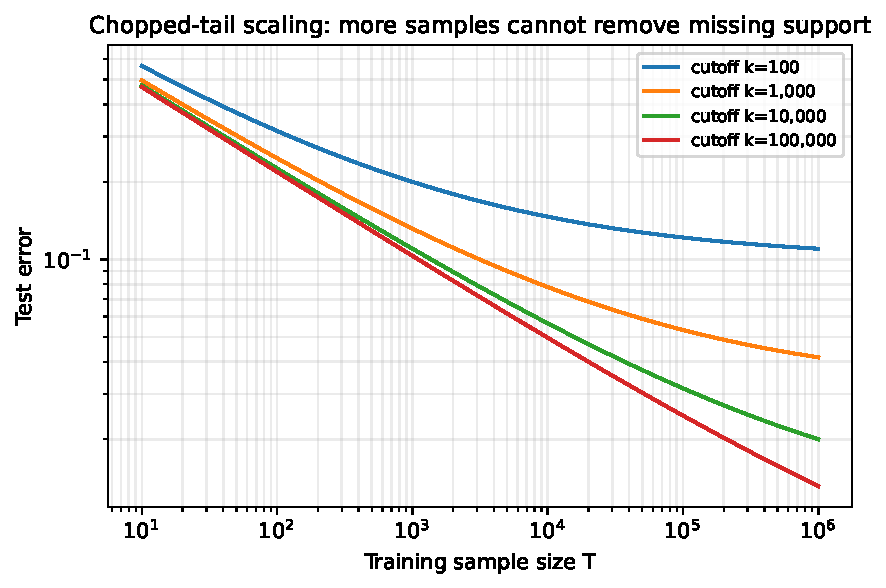
\includegraphics[width=0.78\textwidth]{figures/chopped_tail_scaling.pdf}
\caption{Formula-driven reconstruction of chopped-tail scaling. Increasing $T$ cannot remove a support-dependent floor.}
\label{fig:tails}
\end{figure}

This cell is intentionally simple: it plots the asymptotic expression rather than training a generator. It is useful for reasoning about failure modes, but it does not estimate $k$ for a real model.

\subsection{When synthetic data can help}

The real-synthetic mixing cell uses
\begin{equation}
  E(T_{\rm real},T_{\rm AI},k)
  = (T_{\rm real}+T_{\rm AI})^{-c}+k^{-(\beta-1)}.
\end{equation}
The figure illustrates that synthetic samples can reduce finite-sample error when real data are scarce, while the support floor remains unchanged.

\begin{figure}[H]
\centering
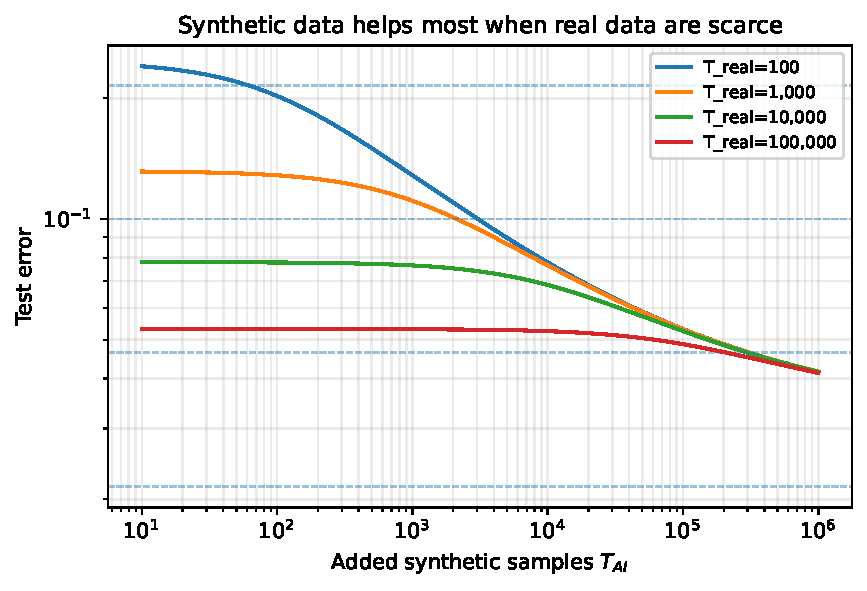
\includegraphics[width=0.78\textwidth]{figures/real_synthetic_mix.pdf}
\caption{Illustrative benefit of synthetic data under real-data scarcity, with an unchanged missing-tail floor.}
\label{fig:mix}
\end{figure}

The operational interpretation is precise: synthetic data can densify a known region of the problem but does not automatically enlarge the set of represented regimes.

\section{Recursive Targets and Verification}

\subsection{Pseudo-label drift}

The notebook represents a true linear relation by $(w_0,b_0)$ and recursively perturbs the previous generation's slope and intercept. This is not a fitted ridge-regression experiment. It is a visual surrogate for the principle
\begin{equation}
  w_0 \rightarrow \widehat w_1 \rightarrow \widehat w_2 \rightarrow \cdots,
\end{equation}
where each model becomes the next model's labeling source. The full theoretical treatment of recursive regression separates bias, variance, noise, regularization, and generational depth \citep{dohmatob2024regression}. The notebook merely makes the direction of drift visible.

\begin{figure}[H]
\centering
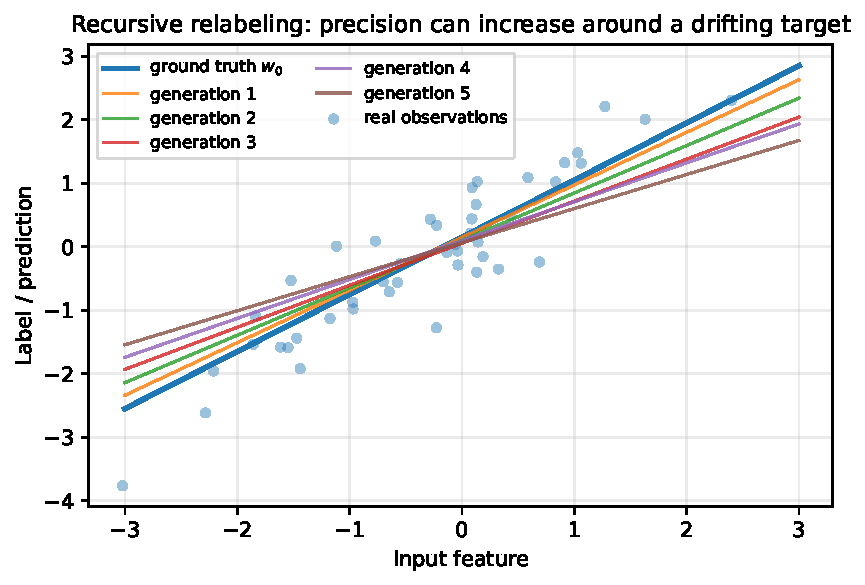
\includegraphics[width=0.78\textwidth]{figures/recursive_relabeling.pdf}
\caption{Conceptual recursive pseudo-label drift. The plotted coefficients are illustrative rather than estimated from data.}
\label{fig:relabel}
\end{figure}

\subsection{Verifier enrichment}

Let a generator be correct with probability $q$. Let a verifier accept a correct candidate with probability $\phi$ and accept an incorrect candidate with probability $\psi$. Bayes' rule gives
\begin{equation}
  \Prob(\mathrm{correct}\mid\mathrm{accepted})
  = \frac{\phi q}{\phi q+\psi(1-q)}.
\end{equation}
For $q=0.20$, the notebook reports the accepted-set precisions in \Cref{tab:verify}.

\begin{table}[H]
\centering
\caption{Verifier enrichment calculated by the notebook.}
\label{tab:verify}
\begin{tabular}{ccc}
\toprule
$\phi$ & $\psi$ & Accepted-set correctness \\
\midrule
0.95 & 0.05 & 82.61\% \\
0.80 & 0.10 & 66.67\% \\
0.60 & 0.20 & 42.86\% \\
0.90 & 0.30 & 42.86\% \\
\bottomrule
\end{tabular}
\end{table}

The final two rows show why acceptance rate alone is insufficient. A verifier that accepts many correct candidates can still be weak if it also accepts too many incorrect ones. This module operationalizes the generate-verify-select-retrain principle studied in verified synthetic-data bootstrapping \citep{feng2025verification}.

\section{MMALS Research Bridge}

The final figure is a deliberately scripted analogy. In the recursive-only scenario, host $H_1$ progressively dominates while $H_2$ and $H_3$ vanish. In the anchored scenario, independent evidence preserves a broader ecology.

\begin{figure}[H]
\centering
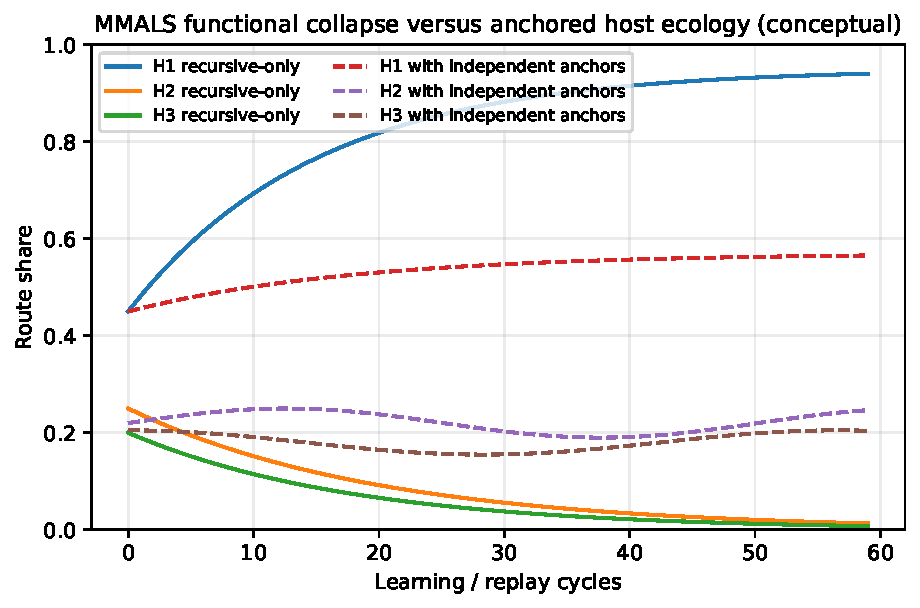
\includegraphics[width=0.82\textwidth]{figures/mmals_host_ecology.pdf}
\caption{Conceptual MMALS route-collapse hypothesis. This figure is not produced from MMALS traces.}
\label{fig:mmals}
\end{figure}

The analogy maps synthetic-data collapse to functional collapse:
\begin{equation}
  \text{frequent modes} \leftrightarrow \text{dominant host or route},
\end{equation}
\begin{equation}
  \text{lost tail} \leftrightarrow \text{lost specialized functions},
\end{equation}
\begin{equation}
  \text{recursive pseudo-labels} \leftrightarrow \text{self-reinforcing replay traces}.
\end{equation}

The notebook therefore formulates, but does not validate, the following hypothesis:
\begin{quote}
A routing ecosystem may become locally stable while globally losing accessible, causally useful functions if its memory and replay are dominated by its own previously selected routes.
\end{quote}

A genuine MMALS experiment must replace scripted shares with observed route traces and must distinguish harmless concentration on simple cases from irreversible loss of functional support.

\section{Reproducibility and Auditability}

The notebook uses only NumPy, pandas, and Matplotlib. A fixed random generator seed, $42$, makes the stochastic relabeling illustration reproducible. The deterministic modules reproduce exactly, modulo library and rendering differences.

A reproducibility claim for this notebook therefore means:
\begin{itemize}[leftmargin=*]
  \item formulas, parameters, and random seeds are visible;
  \item each figure can be regenerated locally;
  \item conceptual figures are labelled as conceptual;
  \item no downloaded model weights or hidden API calls are required;
  \item assumptions can be modified cell by cell.
\end{itemize}

It does not mean:
\begin{itemize}[leftmargin=*]
  \item exact replication of WikiText-103 fine-tuning;
  \item replication of published Llama experiments;
  \item derivation of the full kernel-ridge theorems;
  \item evidence that MMALS currently collapses or resists collapse.
\end{itemize}

\section{From Tutorial to Evidence-Producing Experiment}

The next implementation stage should create a trace-driven notebook with four controlled protocols:
\begin{enumerate}[leftmargin=*]
  \item \textbf{Independent-only:} training and evaluation from externally validated traces;
  \item \textbf{Recursive-only:} new route labels produced by the previous MMALS generation;
  \item \textbf{Fixed anchor:} recursive traces mixed with a fixed real or independently verified anchor;
  \item \textbf{Fresh anchor and verified synthetic:} new independent traces plus synthetic candidates accepted by an external oracle.
\end{enumerate}

The minimum outputs should include:
\begin{itemize}[leftmargin=*]
  \item route distribution and route entropy by regime;
  \item functional tail coverage;
  \item host contribution gain and ablation impact;
  \item route-swap and candidate-permutation sensitivity;
  \item performance on exact repeats, nearby variants, and new compositions;
  \item generation depth, source lineage, freshness, and verifier identity;
  \item compute cost and retained-memory cost;
  \item multi-seed uncertainty.
\end{itemize}

A route should not be preserved merely because it is rare. It should be preserved when it is rare, causally useful, and relevant to a real or stress-tested regime.

\section{Limitations}

The notebook intentionally omits several complexities:
\begin{enumerate}[leftmargin=*]
  \item finite-support normalization slightly modifies ideal asymptotics;
  \item the chopped-tail cells omit unknown multiplicative constants;
  \item pseudo-label drift is scripted rather than estimated;
  \item the verifier module assumes known $q$, $\phi$, and $\psi$;
  \item verifier-induced selection bias is not simulated;
  \item no autoregressive sequence model is trained;
  \item no grokking or late transition is measured;
  \item no real MMALS host, router, memory, or objective is executed.
\end{enumerate}

These omissions are not defects relative to the notebook's purpose. They define the boundary between an explanatory tutorial and a research experiment.

\section{Conclusion}

The companion notebook is best understood as a compact executable argument. It shows that long-tailed data can generate scaling without abstraction, that missing support creates error floors, that synthetic data can help when real data are scarce, that recursive labels can drift, and that a discriminating verifier can enrich a weak generator's outputs. It then translates these mechanisms into a falsifiable MMALS hypothesis about host and route collapse.

Its scientific value lies in disciplined scope. The notebook does not claim that a toy curve is evidence about a production LLM or MMALS release. Instead, it provides a common language, a set of expected signatures, and a precise plan for replacing illustrative curves with real traces, independent anchors, causal interventions, and auditable evidence.

\begin{thebibliography}{9}

\bibitem[Kempe(2024)]{kempevideo2024}
Julia Kempe.
\newblock \emph{Synthetic Data -- Friend or Foe in the Age of Scaling?}
\newblock Public lecture in the IHES Mathematics for and by Large Language Models series, 2024.
\newblock \url{https://www.youtube.com/watch?v=D9x3DT16mGg&list=PLx5f8IelFRgHrJ9W6_fbfO3ahDrXMEIWn}.

\bibitem[Hutter(2021)]{hutter2021learning}
Marcus Hutter.
\newblock Learning curve theory.
\newblock \emph{arXiv preprint arXiv:2102.04074}, 2021.

\bibitem[Dohmatob et~al.(2024a)Dohmatob, Feng, Yang, Charton, and Kempe]{dohmatob2024tails}
Elvis Dohmatob, Yunzhen Feng, Pu Yang, Francois Charton, and Julia Kempe.
\newblock A tale of tails: Model collapse as a change of scaling laws.
\newblock In \emph{Proceedings of the 41st International Conference on Machine Learning}, 2024.

\bibitem[Dohmatob et~al.(2024b)Dohmatob, Feng, and Kempe]{dohmatob2024regression}
Elvis Dohmatob, Yunzhen Feng, and Julia Kempe.
\newblock Model collapse demystified: The case of regression.
\newblock \emph{arXiv preprint arXiv:2402.07712}, 2024.

\bibitem[Feng et~al.(2025)Feng, Dohmatob, Yang, Charton, and Kempe]{feng2025verification}
Yunzhen Feng, Elvis Dohmatob, Pu Yang, Francois Charton, and Julia Kempe.
\newblock Beyond model collapse: Scaling up with synthesized data requires verification.
\newblock In \emph{International Conference on Learning Representations}, 2025.

\end{thebibliography}

\end{document}
